% =========================================================
%  Cabeçalho
% =========================================================

% Define tamanho global de fonte, tipo de documento
\documentclass[12pt]{beamer} % beamer é o pacote para fazer slides de apresentação
\usetheme{Warsaw} % é um dos temas prontos do beamer

% \setbeamercovered{transparent} % nao sei para que serve...

\setbeamertemplate{navigation symbols}{} % remove símbolos de navegação
\setbeamertemplate{headline}{} % remove headline nos frames com a seção-subseção

% Redefine o comando insertshorttitle para adicionar o page-number dos slides
\newcommand{\slidenumber}{\insertframenumber\,/\,\inserttotalframenumber}

\newcommand*\oldmacro{}%
\let\oldmacro\insertshorttitle%
\renewcommand*\insertshorttitle{%
\oldmacro\hfill%
\slidenumber}

% Pacotes usados
\usepackage[utf8]{inputenc} % enconding de caracteres
\usepackage[brazil]{babel}  % locale pt_BR
\usepackage[T1]{fontenc} % importante para não pau nos caracteres...

\usepackage{upquote} % renderiza quote reta ' dentro do verbatim

% Multicolunas, caso for usar
\usepackage{multicol}

% Matemática
\usepackage{amsmath}
\usepackage{amsfonts}
\usepackage{gensymb}

% Imagens
%\usepackage{svg}
\usepackage{graphicx} % para inserir imagens

% Tabelas
\usepackage{booktabs}
\usepackage{caption}

% =========================================================
%  Documento
% =========================================================

% Começo do documento
\begin{document}

% Mostrar tópicos sumário a cada nova seção
\AtBeginSection[]
{
\begingroup
	\renewcommand{\slidenumber}{} % remove pagenumber

	\begin{frame}[noframenumbering]{Tópicos}
		\tableofcontents[currentsection]
	\end{frame}
\endgroup
}

% Mostrar tópicos sumário a cada nova sub-seção
\AtBeginSubsection[]
{
\begingroup
	\renewcommand{\slidenumber}{} % remove pagenumber
	\begin{frame}[noframenumbering]{Tópicos}
		\tableofcontents[currentsection, currentsubsection]
	\end{frame}
\endgroup
}

% =========================================================
%  Capa
% =========================================================

\title{Paradigma de Programação Funcional}
\author[Elias Rodrigues, Vinicius Katata]{Elias Italiano Rodrigues -- 7987251 \and\\
Vinicius Katata Biondo -- 6783972}
\institute[ICMC-USP]{SCC0217 -- Linguagens de Programação e Compiladores\\[\baselineskip]
Instituto de Ciências Matemáticas e de Computação\\
Universidade de São Paulo}
\date{\today} 

\begingroup
	\renewcommand{\slidenumber}{} % remove pagenumber
	\begin{frame}[noframenumbering]
			\titlepage
	\end{frame}
\endgroup

% =========================================================
%  Sumário
% =========================================================

% Cria o Sumário
\begin{frame}{Sumário}
	\tableofcontents
\end{frame}

% Reseta contador de página para 1 (assim não conta a Capa como página)
\setcounter{framenumber}{1}

% =========================================================
%  Conteúdo
% =========================================================

\section{Introdução}

\subsection{O Paradigma}
\begin{frame}{O Paradigma}
	\begin{itemize}
	\setlength\itemsep{1.5em}
		\item O paradigma funcional é baseado em funções matemáticas.

		\item Foi idealizado com o objetivo de criar programas mais legíveis, com funções independentes de contexto, sem efeitos colaterais e mudança de estado durante a execução do programa.

		\item LISP é uma das linguagens mais conhecidas.
	\end{itemize}
\end{frame}

\subsection{Funções Matemáticas}

\begin{frame}{Funções Matemáticas}
	\begin{itemize}
	\setlength\itemsep{1.5em}
		\item Uma função matemática é o mapeamento de elementos de um conjunto em outro conjunto.
		
		\item As expressões matemáticas são expressas por condições e controladas por recursão.

		\item Não dependem de valores externos.

		\item O valor de um parâmetro não é alterado durante a avaliação da função.
	\end{itemize}
\end{frame}

\subsection{Lambda Calculus}

\begin{frame}{\textit{Lambda Calculus}}
	\begin{itemize}
	\setlength\itemsep{1.5em}
		\item Expressões Lambda

		É uma notação para escrever funções sem fazer referência a um nome.

		\begin{equation*}
			\lambda(x) \text{ } x*x*x
		\end{equation*}


		\item \textit{Lambda Calculus}

		É um sistema para definição e aplicação de funções e recursão usando expressões lambda.
	\end{itemize}
\end{frame}

\section{Noções Básicas}

\begin{frame}{Noções Básicas}
	\begin{itemize}
	\setlength\itemsep{1.5em}
		\item Objetivo do paradigma funcional é imitar funções matemáticas; resulta numa abordagem diferente de resolução de problemas.

		\item Não existem o controle de memória, atribuição de dados e estrutura de repetição.

		\item As linguagens funcionais possuem um conjunto primitivo de funções.
	\end{itemize}
\end{frame}

\section{Linguagens}

\begin{frame}{Linguagens}
	Atualmente muitas linguagens funcionais foram desenvolvidas, porém algumas tomaram um rumo mais parecido com as linguagens imperativas, adquirindo ferramentas que aumentam a eficiência de execução. LISP é um exemplo.\\[\baselineskip]

	\begin{itemize}
		\item ML

		\item Caml, SML, F\#, Scheme
	\end{itemize}
\end{frame}

\section{LISP}

\subsection{Listas}

\begin{frame}{LISP}{Listas}
	\begin{itemize}
	\setlength\itemsep{1.5em}
		\item Não existe tipagem de dados, porém existe dois tipos de objetos de dados: átomos e listas.

		\item Uma lista é composta por dois campos: o primeiro é o dado do elemento e o segundo pode ser um ponteiro para o próximo elemento ou uma lista vazia.
	\end{itemize}
\end{frame}

\begin{frame}{LISP}{Listas}
	\begin{center}
	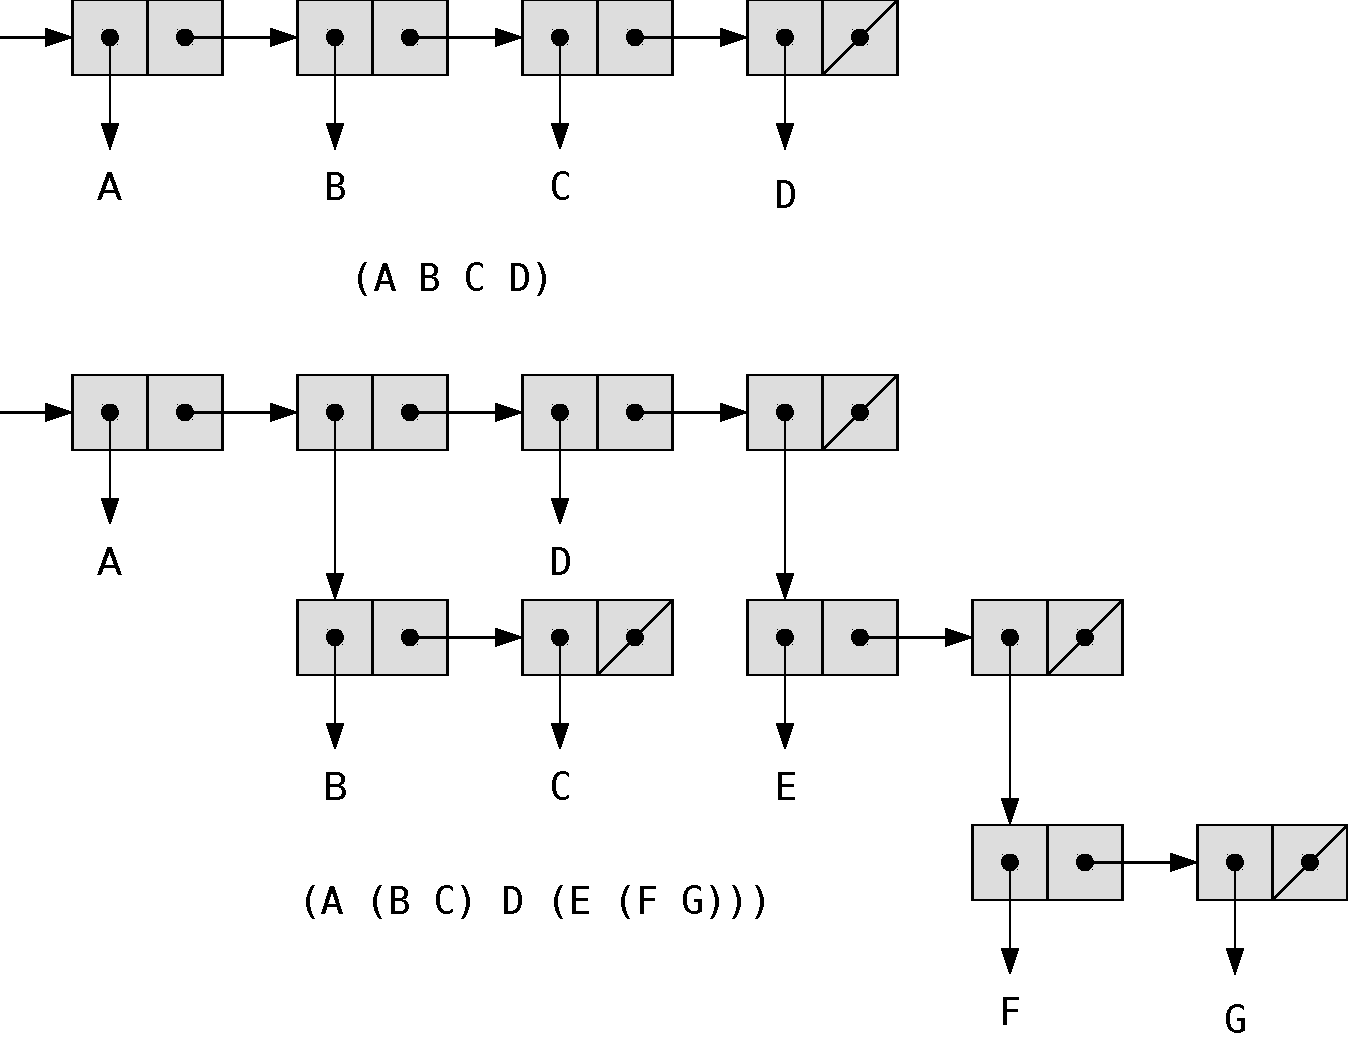
\includegraphics[scale=.4]{../listas.pdf}
	\end{center}
\end{frame}

\begin{frame}[fragile]{LISP}{Listas}
	Funções do LISP também são expressas no formato de listas.\\[\baselineskip]

	\begin{block}{Exemplo}
		\begin{verbatim}
		(defun double (x)
		    (+ x x)
		)
		\end{verbatim}
	\end{block}
\end{frame}

\subsection{Funções Primitivas}

\begin{frame}[fragile]{LISP}{Funções Primitivas}
	Existem dois tipos de funções: as primitivas e as definidas pelo usuário.

	\begin{itemize}
		\item Algumas primitivas sobre números:

		\texttt{+}, \texttt{-}, \texttt{/}, \texttt{*}\\[\baselineskip]

		\begin{block}{Exemplo}
			\begin{verbatim}
			(* 2 2)
			\end{verbatim}
			Saída: \texttt{4}
		\end{block}

	\end{itemize}
\end{frame}

\begin{frame}[fragile]{LISP}{Funções Primitivas}
	\begin{itemize}
	\setlength\itemsep{1.5em}
		\item Algumas funções sobre listas:

		\texttt{first}, \texttt{last}, \texttt{rest}, \texttt{append}, \texttt{list}\\[\baselineskip]

		\begin{block}{Exemplo}
			\begin{verbatim}
			(first '(A B C D))
			\end{verbatim}
		\end{block}

		\item Aspa simples também é uma primitiva.

	\end{itemize}
\end{frame}

\subsection{Predicados}

\begin{frame}[fragile]{LISP}{Predicados}
	\begin{itemize}
	\setlength\itemsep{1.5em}
		\item Predicados são funções primitivas que retornam verdadeiro ou falso.

		\item Verdadeiro é denotado por \texttt{T} e falso por \texttt{NIL}.\\[\baselineskip]
		
		\begin{block}{Exemplo}
			\begin{verbatim}
			(symbolp +)
			\end{verbatim}
			Saída: \texttt{T}
		\end{block}
	\end{itemize}
\end{frame}

\begin{frame}[fragile]{LISP}{Predicados}
	\begin{itemize}
	\setlength\itemsep{1.5em}
		\item Outros predicados muito utilizados são os relacionais:\\
		\texttt{>}, \texttt{>=}, \texttt{<}, \texttt{<=}, \texttt{=}, \texttt{/=}\\[\baselineskip]

		\begin{block}{Exemplo}
			\begin{verbatim}
			(< 671 9)
			\end{verbatim}
			Saída: \texttt{NIL}
		\end{block}

	\end{itemize}
\end{frame}

\subsection{Estruturas de Controle}

\begin{frame}[fragile]{LISP}{Estruturas de Controle}
	LISP provê duas formas de controlar e organizar o fluxo de execução: condições e recursão.\\[\baselineskip]

	\begin{block}{Exemplo}
		\begin{verbatim}
		(defun list-nth (n L)
		    (cond
		        ((null L) nil)
		        ((zerop n) (first L))
		        (t (list-nth (- n 1) (rest L)))
		    )
		)
		\end{verbatim}
	\end{block}
\end{frame}

\section{Common Lisp}

\begin{frame}[fragile]{Common Lisp}
	\begin{itemize}
	\setlength\itemsep{1.5em}
		\item É um dialeto de LISP onde foram implementadas ferramentas de linguagens imperativas:\\
		\texttt{if}, \texttt{case}, \texttt{while}, \texttt{for}, etc\\[\baselineskip]

	\begin{block}{Exemplo}
		\begin{verbatim}
		(defun fac (n)
		    (if (= n 0) 1
		        (* n (fac (- n 1)))
		    )
		)
		\end{verbatim}
	\end{block}
	\end{itemize}
\end{frame}

\section{Haskell}

\begin{frame}[fragile]{Haskell}
	\begin{itemize}
	\setlength\itemsep{1.5em}
		\item É uma linguagem de programação puramente funcional, ou seja, não possui expressões ou declarações que tem efeitos colaterais.\\[\baselineskip]

	\begin{block}{Exemplo}
		\begin{verbatim}
		fact n
		   | n == 0 = 1
		   | n == 1 = 1
		   | n  > 1 = n * fact(n - 1)
		\end{verbatim}
	\end{block}
	\end{itemize}
\end{frame}

\section{Conclusão}

\begin{frame}{Conclusão}
	\begin{itemize}
	\setlength\itemsep{1.5em}
		\item Com base na não dependência de contexto, testes sobre funções são de fácil implementação.

		\item Porém, a aplicação pura do paradigma funcional é apenas para sistemas muito específicos.

		\item Além disso, para leigos em definições matemáticas haverá uma certa dificuldade inicial na modelagem de soluções para os problemas.
	\end{itemize}
\end{frame}


% =========================================================
%  Referências
% =========================================================

% Começo das Referências
\begin{frame}{Referências}
	\begin{thebibliography}{9}

		\bibitem{bib:livro}
			SEBESTA, Robert W. \textit{Concepts of Programming Languages}. United States of America: Pearson, 10ed., 2010.

	\end{thebibliography}
\end{frame}
% Fim das Referências

\end{document}
% Fim do documento
